\documentclass{article}
\usepackage[utf8]{inputenc}
\usepackage[english]{babel}
\usepackage[nottoc]{tocbibind}
\usepackage{indentfirst}
\usepackage{mathtools,xparse}
\usepackage{appendix}
\usepackage{eucal}
\usepackage{amsmath,amsfonts,amssymb,amsthm,amssymb}
\usepackage{bbm}
\usepackage{commath}
\DeclareUnicodeCharacter{FB01}{fi}


\title{Misalignment Recognition Using Markov Random Fields with Fully Connected Latent Variables for Node Movement Detection in Noisy and Reverberant Acoustic Environment }
\author{Gabriel F Miller}
\date{February 2020}

\begin{document}

\maketitle

\section{Background}

Sound source localization is a topic that has been covered in great detail for many years and still remains a burgeoning field of study. Some of the different applications that continue to drive the need for more robust and efficient estimators include video conferencing, automatic camera steering, smart home technology and speaker separation. In this paper, we consider the problem of source localization with an ad-hoc microphone array network and multiple sources in noisy and reverberant environments. In particular, we consider the situation in which any given microphone array is moving and how to best update the sensor network's source position estimate in real time.

In the past, traditional localization methods have generally been categorized in three different groupings. One such being those based on the maximization of a steered response power (SPR) of a beamformer output whereby the measured signals are  filtered and summed together and the maximum likelihood criterion is used to determine the output power of a beamformer steered to different locations \cite{ROS_multipleEmitterLocation}. There are also high-resolution spectral estimation techniques, such as the multiple signal classification (MUSIC) method \cite{KY_music}, or the estimation of signal parameters via rotational invariance (ESPRIT) \cite{RR_esprit} algorithm. Both are based on the spectral analysis of the correlation matrix of measured signals. A third method is a dual-stage approach relying on a time difference of arrival (TDOA) estimate. In the first stage, the TDOAs of different pairs of microphones are estimated and collected with each reading of the TDOA said to correspond with the single-sided hyperbolic hyperplanes (in 3D) representing possible positions. The intersection of these hyperplanes yields the estimated position. Some classic TDOA estimation methods of this type include the generalized cross-correlation (GCC) algorithm \cite{CK_generalizedCorrelationMethodforTimeDelay}. 

What most of these methods have in common, is that they rely on physical models that are dependent on assumptions regarding the propagation model and the statistics associated with signals that are trying to be localized. These physical models though, have a level of complexity that make robust estimates very difficult to acquire. For example, in an  environment with adverse audio conditions, such as added noise that is non-stationary, or a room with a non-uniform structure, composed of many different materials with varying reflective qualities, getting a robust estimate becomes more difficult.

More recently, there has been a new found interest in estimating an acoustic source based off of learning-based methods. These methods look to estimate a position directly from data (opposed to any physical model). Both supervised and unsupervised methods have been introduced, where supervised methods imply that in the training phase, microphone measurements of sources are known as well as the microphone measurements, versus unsupervised methods where only the measurements are known. Methods have been proposed to localize using learning-based methods for both the binaural and multiple microphone array cases \cite{AD_2dSoundsourceLocalBinMani, AD_VariEMforBinSoundSepAndLocal, AD_acousticSpaceLearningforSoundSep}. 

Different features have also been explored for both cases. In \cite{TM_probModelRobustLocalizationBinauralAudioFront}, the authors used a Gaussian Mixture Model (GMM) based approach to learn the azimuth-dependent distribution of the binaural feature space. In \cite{XX_learningApproachDoaEstimation} the authors used GCC-based feature vectors for training a multi-layer perceptron neural network that output the source direction of arrival (DOA). In \cite{BLG_rtfModelingSupervisedSourceLocalization}, the authors used a power spectral density (PSD)-based feature vector with a slightly different approach. In particular, the authors introduced a supervised method based on manifold learning. The goal in this method was to recover the controlling parameter of the acoustic impulse response (AIR).

\section{Procedural Overview} 
In this paper we consider a similar approach to estimating the position of an acoustic source using multiple microphone arrays as that done in \cite{LG_semisupervisedSourceLocalization}. In their work, the authors look to estimate a target function using a Bayesian inference framework described by a likelihood function and prior probability. In essence, the likelihood function measures the correspondence of the target function to the labelled examples, while the prior probability reflects our prior belief regarding the distribution of the target function. The authors utilize a feature vector based on relative transfer function (RTF) estimates as their target function, and a so-called manifold-based prior, meaning it relies on the geometric structure of RTF samples implied by labelled and unlabelled samples. These samples are used in a training phase to gain information on the acoustic characteristics of a given environment and to derive parameters that can be used in inferring the position during a test phase. The general procedure is as follows:\\\\\\ \textbf{Training Phase}
\begin{itemize}
  \item \textit{RTF estimation:} We first estimate RTF samples for both labelled and unlabelled sources. Samples are recorded for each microphone array.
  \item \textit{Covariance Estimation:} The covariance matrix, which we describe in more detail below, is calculated and associates the different samples recorded at each array. It is with the inverse covariance matrix (the precision matrix), that we estimate the position of a test source.
\end{itemize}
\textbf{Test Phase}
\begin{itemize}
  \item \textit{RTF estimation:} We first estimate the RTF associated with a given test source.
  \item \textit{Covariance Estimation:} A covariance vector is calculated relating the test RTF measured at each array with those used for training. 
  \item \textit{Adaptation:} Here we adapt the the precision matrix to account for the new RTF (test) sample. 
  \item \textit{Position Estimation:} The updated precision matrix is used to estimate the position of the test source.
\end{itemize}

\section{Setup}

\begin{figure}[htbp]
\centering
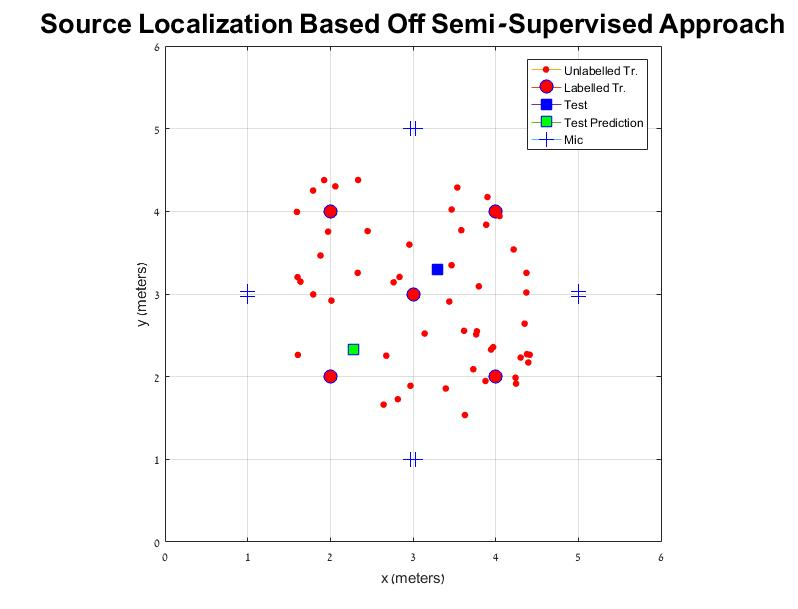
\includegraphics[width=0.6\linewidth]{figures/environment_overview.jpg}
\caption[Source Localization Based Off Semi-Supervised Approach]{Overview of the simulated room used for estimating a test audio source based on a semi-supervised approach using labelled and unlabelled sources.}
\label{fig:room_overview}
\end{figure}

We look to estimate a single source position \textbf{q} = [\textit{$q_x$}, \textit{$q_y$}, \textit{$q_z$}]$^T$ using an ad-hoc network of microphone arrays where each array consists of 2 microphones spaced 20 cm apart (figure 1). The source produces an unknown speech signal $\textit{s(t)}$, which is recorded by all microphones. The signal received by the $\textit{i}$th microphone of he $\textit{m}$th pair is given by: 

\begin{equation} \label{source_eqn}
    \begin{aligned}
        \textit{{y}$_i^m(t)$} = \textit{{a}$_i^m$(t,\textbf{q})} * \textit{s(t)} + \textit{{u}$_i^m$(t)}
    \end{aligned}
\end{equation}

Here, \textit{m} references the microphone array and \textit{i} specifies one of the two microphones in the \textit{m}th array. Additionally, \textit{${a}_i^m$(t,\textbf{q})} is the acoustic impulse response (AIR) relating the source at position \textbf{q} and the \textit{i}th microphone, and \textit{${u}_i^m$(t)} is an additive noise signal which corrupts the corresponding measured signal. Linear convolution is denoted by *. We can see that the information required for localization is embedded in the AIR, and is independent of the source signal. Thus the goal presented in the semi-supervised approach to localization is to extract a feature vector $\textbf{h}^\textit{m}$ that depends solely on the two AIRs of the corresponding node. 

As noted, the feature vector used is the so called RTF. RTFs are typically represented in a high dimensional space, with a large number of coefficients to allow for the full description of the acoustic paths which represent a complex reflection pattern. In reality though, the RTFs are controlled by a small set of parameters, such as room dimensions, reverberation time, location of the source and microphone arrays, etc. This of course naturally leads to the assumption that a large part of the information that RTFs hold are confined to a low dimensional manifold. The mapping function used to relate the high dimensional RTF samples and the source positions, is modelled as a Gaussian process with a covariance function that was built based on a Gaussian kernel function. 

We define the function $\textit{${f}^m_a$} : \textit{$M_m$} \rightarrow {\rm I\!R}$ for \textit{a} $\in \{\textit{x,y,z}\}$ whereby \textit{${f}^m_a$} maps an RTF sample, $\textbf{h}^\textit{m}$, associated with node \textit{m} to the corresponding coordinates of the source position. In particular, we denote the position evaluated by \textit{${f}^m_a$} for the RTF sample $\textbf{h}^\textit{m}$ as \textit{${p}_i^m$} where \textit{i} here now references a given source position that yields a given RTF sample.

It is assumed that \textit{${p}^m$} follows a Gaussian process. Gaussian processes (GPs) are used in practice as a method of analyzing data in the supervised learning context \cite{CER_gaussianProInML}. Specifically, GPs assume a prior distribution to be used for Bayesian inference, meaning the distributions are updated over time based off new information that comes along. By definition, GPs are a collection of Random Variables which have a joint Gaussian distribution, and can be thought of as distributions over functions. They are fully specified by their mean and covariance, and are processed over functions (rather than vectors as is the case with the Gaussian distribution). There are many benefits to GPs; particularly, while general parametric models can lack in expressive power or intelligibility, GPs are thought to excel. In addition, GPs are nice in that they essentially fit the data and complexity terms automatically. Weights do not require to be trained, and cross validation is also not necessary. By modelling the mapping function from the RTF samples to the source positions as a GP, we have an easy and intuitive way of updating the covariance matrix as new information is presented. We assume a zero-mean Gaussian process for simplicity which essentially enforces the assumption that all possible source positions are distributed around some origin. 

In order to express the complex relation tying together all the information obtained at each node, we introduce a kernel based covariance matrix, whereby each element represents a pairwise affinity between two RTF samples. In particular, we express the relationship between two processes as follows: 

\begin{equation} \label{cov_element}
    \begin{aligned}
        cov(\textit{{p}$_{l_i}^m$}, \textit{{p}$_{l_j}^m$}) \equiv \displaystyle\sum_{i=1}^{{n}_D} \textit{{k}$_m$}(\textbf{h}_{l_i}^\textit{m},\textbf{h}_i^\textit{m})\textit{{k}$_m$}(\textbf{h}_{l_j}^\textit{m}, \textbf{h}_i^\textit{m})
    \end{aligned}
\end{equation} where we note that \textit{r} and \textit{l} denote ascription to labelled source positions, \textit{n$_D$} denotes the total number of RTF samples used in training (including both labelled and unlabelled samples), and \textit{k$_m$} (\textbf{h}$_i^\textit{m}$, \textbf{h}$_j^\textit{m}$) is a standard pairwise kernel function \textit{k$_m$}: \textit{M$_m$} $\times$ \textit{M}$_m$ $\rightarrow$ ${\rm I\!R}$. The authors here use the commonly known Gaussian kernel:

\begin{equation} \label{gauss_kern}
    \begin{aligned}
        \textit{k$_m$}(\textbf{h}_i^\textit{m}, \textbf{h}_j^\textit{m}) = exp(-\frac{\norm{\textbf{h}_i^\textit{m} - \textbf{h}_j^\textit{m}}^2}{\textit{$\varepsilon_m$}})
    \end{aligned}
\end{equation}

With both of these definitions, we can now define the manifold-based kernel:

\begin{equation} \label{mani_kern}
    \begin{aligned}
        \textit{$\tilde{k}_m$}(\textbf{h}_i^\textit{m}, \textbf{h}_j^\textit{m}) \equiv cov(\textit{{p}$_{l_i}^m$}, \textit{{p}$_{l_j}^m$})
    \end{aligned}
\end{equation}

In practice this manifold kernel is useful for identifying structural similarities in non-linear classification problems. The methods used here are similar to those introduced in \cite{semiSuperGaussProClass}. These methods are based on an analysis scheme that considers a low-dimensional intrinsic geometry driven by measurements. The analysis relies on a data set with many features that can be expressed by a lower dimensional representation, and acts to preserve the geometric relationship when mapping from the original space to the lower dimensional one. The hope is that this new representation will capture the main structures of the data in few dimensions, thereby achieving dimensionality reduction \cite{diffMapsSigProc}. In particular, the semi-supervised GP method (SSGP) can be seen as providing a Bayesian analogue of Laplacian Support Vector Machines (LapSVM) and Laplacian Regularized Least Squares (LapRLS). For background, we consider a more general setup to the one that we've described so far, namely a symmetric positive semi-definite function \textit{K}($\cdot$,$\cdot$) is used as the covariance function of a Gaussian process and also as a kernel function of a deterministic Reproducing Kernel Hilbert Space (RKHS) \textit{H} of functions that map a given pair of inputs from a given domain to the RKHS: \textit{X} $\rightarrow {\rm I\!R}$. It is said the RKHS and the GP associated with the kernel function, \textit{K}($\cdot$,$\cdot$), are closely related through a classical isometry between \textit{H} and a Hilbert space of random variables spanned by the GP that are of the form $\sum_{k}$ $\alpha_k$\textbf{$f_{x_{k}}$}. The norm, $\left\| \textbf{f} \right\|_{\textbf{H}}$ can be interpreted as a smoothness measure over functions \textbf{f} in \textit{H}. Learning algorithms are thus developed based on minimizing functions of the form: \textit{V}(\textbf{f}, \textit{$X_{L}$}, \textit{$Y_{L}$}) for some cost function \textit{V}, functional  \textbf{f} and input, output pair \textit{$X_{L}$}, \textit{$Y_{L}$} respectively. Minimizing said cost function is generally what is done in both Regularized Least Squares (RLS) and Support Vector Machine (SVM) based problems. One of the benefits of the semi-supervised approach, is that unlabelled data is also put to use. That is to say, unlabelled data may suggest alternate measures of complexity, such as smoothness with respect to data manifolds or clusters, that can be used to re-structure \textit{H} by refining the norm. It does so by using a combination of both labeled data, \textit{$X_{L}$}, and unlabeled data, \textit{$X_{U}$}, with $\textit{$X_{L}$} \cup \textit{$X_{U}$} = \textit{$X_{D}$}$. Now with both sets of data, and the aforementioned manifold kernel, we are able to measure smoothness with respect to the manifold and infer similarities between new test samples and clusters defined in the lower dimensional space \cite{semiSuperGaussProClass}. 

When applying SSGP classification to source localization, in order to build the covariance matrix interlacing the relationship between RTF samples, we rely heavily on the labelled points. In particular, the pairing, \{\textbf{h}$_\textit{i}$, $\bar{\textit{p}_\textit{i}}$\}$^\textit{n$_L$}_{\textit{i}=1}$ for \textit{n$_L$} labelled points serve as a sort of anchor that helps interpolate a realization of the process \textit{p}. Note,

\begin{equation} \label{noisy_pos}
    \begin{aligned}
       \bar{\textit{p$_i$}} = \textit{p$_i$} + \textit{$\eta_i$}; i = 1,...,\textit{n$_L$}
    \end{aligned}
\end{equation} \\denotes a positional estimate with $\textit{$\eta_i$}\backsim\mathcal{N}\left(0, \textit{$\sigma^2$}\right)$ being i.i.d. Gaussian noises, independent of \textit{p$_i$}. Note that both \textit{p$_i$} and \textit{$\eta_i$} are independent, and jointly Gaussian implying $\bar{\textit{p}_\textit{i}}$ is also jointly Gaussian.

We now show how we can build a kernel-based covariance matrix, utilizing the information gained from both labelled and unlabelled training points. We first formally define the kernel covariance matrix, \textit{$\tilde{\Sigma}_L$} $\subseteq \mathbb{R}^{\textit{n$_L$}\times\textit{n$_L$}}$, that consists of elements based off kernel relations we have already introduced. In particular we say 

\begin{equation} \label{cov_element}
    \begin{aligned}
        {\left(\textit{$\tilde{\Sigma}_L$}\right)}_{l_i,l_j}= cov(\textit{p}_{l_{i}}, \textit{p}_{l_{j}}) &\equiv  \textit{$\tilde{k}$}\left(\textbf{h}_{l_{i}}, \textbf{h}_{l_{j}}\right) \\&= \frac{1}{\textit{M}^2} \sum_{d=1}^{{n}_D}\sum_{q,w=1}^{M} \textit{k$_q$}\left(\textbf{h}_{{l}_i}^q, \textbf{h}_d^q\right)\textit{k$_w$}\left(\textbf{h}_{l_j}^w, \textbf{h}_d^w\right) 
    \end{aligned}
\end{equation}

We note here that \textit{d} indicates indexing over all RTF samples (labelled and unlabelled), \textit{q}, \textit{w} refer to microphone arrays, and \textit{l$_i$} and \textit{l$_j$} refer to labelled points. It should now be clear how the labelled points and their associated transfer functions play as a sort of anchor for realizing a given GP, while the unlabelled points still play a key role in re-structuring the matrix based off additional information. Overall, every node can be seen as representing a different view point, which is realized by the structure of the associated manifold \textit{M$_m$}. Moreover, we can view each kernel matrix \textbf{K$^\textit{m}_\textit{H}$}, as a matrix containing the weights associating the RTF samples of different nodes. This would then indicate, that we are essentially producing via the covariance matrix a discrete representation of the \textit{m}th manifold by a graph \textit{G$^m$}. Interestingly, with some simple derivations, one can find an alternative definition for the general covariance matrix, \textbf{$\tilde{\Sigma}$}$_H$, namely:

\begin{equation} \label{kernMat_cov}
    \begin{aligned}
        \textit{$\tilde{\Sigma}$}_\textit{H} = \frac{1}{\textit{M}^2} \sum_{q,w=1}^{M} \textbf{K}^q_\textit{H}\textbf{K}^w_\textit{H}
    \end{aligned}
\end{equation}

Here, we note that each element in \textbf{K}$^m_H$ for a given microphone array is calculated via [\ref{gauss_kern}]. This formulation allows us to see more clearly how the correlation between two nodes is defined. By multiplying the kernels of each two nodes as indicated in [\ref{kernMat_cov}], we are essentially averaging out incoherent node-specific variables and are left with only the common variable, which is the position of the source. That is to say, when measuring the correlation between two nodes the common source of variability is emphasized, i.e. the source position, and we suppress artifacts and interference, which are node specific effects. This perspective provides a justification to the averaging over different nodes as well as over different samples, constituting a robust measure of correlation between samples in terms of the physical proximity between the corresponding source positions. 

With the derivation of the covariance matrix containing the weights relating the viewpoints of each array, it is now possible to provide a robust estimate of a source test position given an RTF sample, \textbf{h}$_\textit{t}$. This is done, by updating our weights in a Bayesian manner based off the information provided by a new sample. We do not go into extensive detail here on the specifics of this procedure, as we provide a modified approach to the updating process in the context of our newly defined problem below. For more details for the updating process in the context of a static microphone array network, please refer to \cite{LG_semisupervisedSourceLocalization}. 

We do reference here though, some of the equations that allow us to estimate a test position. Consider some new test RTF sample, \textbf{h}$_t$ $\in$ \textit{H}$_T$ that is the product of some unknown source at an unknown location. The estimation is based on the posterior probability:

\begin{equation} \label{posterior}
    \begin{aligned}
        Pr\left(\textit{p$_t$} \equiv \textit{f}\left(\textbf{h}_\textit{t}\right) \mid \textit{P$_L$}, \textit{H$_L$} \right)
    \end{aligned}
\end{equation}

We thus construct an estimate of some \textit{$\hat{p}_t$} based on the maximum a posteriori probability (MAP) estimator which is equivalent to the minimum mean squared error (MMSE) estimator in the Gaussian case. To do so, first note that the concatenation of all labelled training positions, \textbf{p}$_\textit{L}$ = $\left[\textit{$\bar{p}_1$},...,\textit{$\bar{p}_{n_L}$}\right]^T$ are jointly Gaussian with:

\begin{equation} \label{concat_pos_est}
    \begin{bmatrix}
        \textbf{p$_L$}\\
        \textit{p$_t$}
    \end{bmatrix}\rvert \textit{H$_L$} \backsim \mathcal{N}\left(\textbf{0}_{\textit{n}_L}, 
    \begin{bmatrix}
        \textbf{$\tilde{\Sigma}$}_\textit{L} + \textit{$\sigma^2$}\textbf{I}_{\textit{n$_L$}} & \textit{$\tilde{\Sigma}$}_\textit{Lt}\\
        \textbf{$\tilde{\Sigma}$}_\textit{Lt}^T & \textit{$\tilde{\Sigma}$}_\textit{t}
    \end{bmatrix}
    \right)
\end{equation}

Here, we have already defined \textbf{$\tilde{\Sigma}_{L}$} as an $\textit{n$_L$} \times \textit{n$_L$}$ covariance matrix defined over function values at labelled points. Additionally, we define \textit{$\tilde{\Sigma}_{Lt}$} to be an $\textit{n$_L$} \times 1$ covariance vector between the function values at \textit{H}$_L$ and some function value at a test point \textit{p$_t$}, \textit{$\tilde{\Sigma}_t$} is the variance of \textit{p$_t$},  \textit{$\sigma^2$} is the variance associated with the Gaussian noise, and \textbf{I$_{\textit{{n}$_L$}}$} is the $\textit{n$_L$} \times \textit{n$_L$}$ identity matrix. With this in mind, we can now define the positional optimal estimate of some test position,

\begin{equation}\label{test_est}
    \begin{aligned}
        \textit{$\hat{p}_t$} = \mu_{cond} = \textit{$\tilde{\Sigma}_{Lt}$}\textbf{$\tilde{p_L}$}
    \end{aligned}
\end{equation}

Here, $\mu_{cond}$ is the mean of the multivariate Gaussian distribution,\\ $\textit{Pr}\left(\textit{p$_t$}\mid\textit{P$_L$},\textit{H$_L$}\right))$, and is calculated by multiplying the test covariance vector by a vector of weights, \textbf{$\tilde{p}_L$}, which are independent of a given test sample and are obtained via the inverse covariance matrix with some added noise; \textbf{$\tilde{p}_L$} = $\left(\textit{$\tilde{\Sigma}_L$} + \textit{$\sigma^2$}\textbf{I}_{\textit{n$_L$}}\right)^{-1}$\textbf{p}$_L$. For convenience, we refer to $\left(\textit{$\tilde{\Sigma}_L$} + \textit{$\sigma^2$}\textbf{I}_{\textit{n$_L$}}\right)^{-1}$ as $\Gamma_L$ for the remainder of the paper.


\section{Movement Detection}
In the case of estimating a source with a moving microphone array, there are several components that need to be considered. Firstly, there must be some way of knowing when one or multiple of the microphone arrays move, as well as knowing which array it was. Moreover, there must be a way in real time, to update the estimate. For the first two problems, we consider a technique recently introduced in the field of robotics for recognizing sensor misalignment via Markov Random Fields (MRFs) with fully connected latent variables \cite{NA_misalignmentRecMRFsFcn}. In the paper, the authors consider the problem of discerning whether aligning individual sensor readings to localize a given object. In particular, a set of sensors are used to compare physical readings of an open space with a map of said space that is known beforehand. The method implemented takes as input the residual error of a given sensor reading and that of the true map, and estimates the posterior class probabilities of each sensor measurement via an MRF with fully connected latent variables (FCLV). Rather than taking each reading independently, the MRF allows for consideration of the entire network relationship to indicate whether sensor measurements are aligned, misaligned or obtained from unknown obstacles (not included in the original mapping). The posterior probabilities output from the MRFs with FCLVs are used to indicate when there is a misalignment among the sensors, and to detect which particular sensor led to localization failure.

To better understand the approach of the authors and MRFs, we first introduce the general Naive Bayes model:

\begin{equation} \label{naiveBayes}
    \begin{aligned}
        \textit{p}\left(\textbf{$\overrightarrow{y}$}\mid\textbf{$\overrightarrow{x}$}\right) = \prod_{i=1}^n \textit{p}\left(\textit{y}_i\right)\textit{p}\left(\textit{x}_i\mid\textit{y}_i\right)
    \end{aligned}
\end{equation} where \textit{p}$\left(\textit{x}_i\mid\textit{y}_i\right)$ is referred to as the generative model in that it describes the process of generating sensor measurements under different worlds \textbf{y}, and \textit{p}$\left(\textit{y}_i\right)$ is what is known as the prior, i.e. the specification of our willingness to assume that \textbf{y} is the reality in the so-called world, before any additional data is received \cite{ST_roboticMappingSurvey}. The Naive Bayes model can be useful in that it is tractable in computing likelihoods of different observations based on evidence. However, the model cn be limited as it assumes independence of all observations, hence the moniker, "naive". Solutions to this are addressed with Bayesian Networks. These networks are a commonly used way to represent a graphical model whereby a network is described by nodes and edges \cite{JSY_understandBeliefPropAndGeneral}. Each node signifies a hidden state that defines the underlying structure of a given network. The edges indicate a conditional probability that describes the relationship between all of the different nodes. These edges also encompass a directional relationship from a so-called parent node to their children, with Bayesian Networks being directed and acyclic, meaning the directionality imposed in the network does not loop around in a cycle. Bayesian networks can be fully described by the following joint probability function: 

\begin{equation} \label{bayesNet}
    \begin{aligned}
        \textit{p}\left(\textit{x$_1$}, \textit{x$_2$},...,\textit{x$_N$} \right) = \prod^\textit{N}_\textit{i=1} \textit{p}\left(\textit{x$_i$}\mid\textit{Par}\left(\textit{x$_i$}\right)\right)
    \end{aligned}
\end{equation} where \textit{Par}$\left(\textit{x}_i\right)$ denotes the state of the parents of node \textit{i}. Note that if node \textit{i} has no parents, we take \textit{p}$\left(\textit{x}_i\mid\textit{Par}\left(\textit{x}_i\right)\right)$ = \textit{p}$\left(\textit{x}_i\right)$. The way in which these joint probabilities are utilized of course is to define certain probabilistic relations between different nodes and their likelihood of causal impact in a given network. This is done in practice by computing certain marginal probabilities, or beliefs as they are often referenced in pertinent literature, while the computational aspect is referred to as inference. Inference here is an apt description of the process, as Bayesian Networks assume not only a set of observations, but also a set of hidden variables, or states that govern the relationship between different sub-networks of nodes. Theoretically, marginal probabilities are defined in terms of sums over all the possible states of all the other nodes in the system. For example, if we want the marginal probability of a node \textit{p}$\left(\textit{x}_i^*\right)$, we compute

\begin{equation} \label{marginalization}
    \begin{aligned}
        \textit{p}\left(\textit{x$_i^{*}$}\right) = \sum_\textit{x$_1$}\sum_\textit{x$_2$} \cdots \sum_\textit{x$_{i-1}^{*}$} \textit{p}\left(\textit{x$_1$}, \textit{x$_2$},...,\textit{x$_i^{*}$} \right)
    \end{aligned}
\end{equation}

There are two competing issues that we now address. We first introduced [\ref{naiveBayes}] and noted how the independence assumption could be lacking in fully describing the relation between our observations and also the potential causal effects on the probability of a given observation occurring, if another observation is realized. With Bayesian networks, there is another issue, namely tractability. For small Bayesian networks, marginalization can be done directly and the summation over all possible states presents no issue. For bigger networks however,the number of terms in the sums grows exponentially with the the number of hidden nodes in the network. It is here where MRFs, and the approximation algorithms developed to label them, are particularly potent. Specifically, MRF theory provides a convenient and consistent way of modeling context dependent entities, in particular, spatially correlated features \cite{LI_mrfModelingCompVis}. Specifically, MRF theory tells us how to model the \textit{a priori} probability of contextual dependent patterns, such as a class of textures, and an arrangement of object features. This is achieved by characterizing mutual influences among such entities using \textit{a posteriori} probabilities based on original assumptions, and new observations. Computationally, MRFs can be implemented in a local and massively parallel manner. 

The general idea behind MRFs is as follows. We first observe some quantities \textit{y}$_i$ and want to infer some other quantities about the underlying scenario (which we refer to as hidden variables) and denote as \textit{x}$_i$. Note that the index \textit{i} could be thought of as representing a node position, or the position of a small patch of nodes. We now define $\phi_i\left(\textit{x$_i$},\textit{y$_i$}\right)$, which we refer to as the evidence of \textit{x}$_i$ i.e. a probabilistic relation between a hidden state and our observations. It is with the evidence that we can come to understand what makes MRFs unique; in particular, it is the ability to quantify the relationship between hidden states and observations. It's worth noting that for one of the more common use cases of MRFs, computer vision and robotics, the function usually denotes a disparity between an observation and a given set of labels \cite{YB_fastApproxEnergyMinGraphCuts}. E.g. for image restoration, the observations are typically a pixel intensity while the labels are a discrete and often smaller set of possible intensities, and in \cite{NA_misalignmentRecMRFsFcn}, the labels used were localization estimates from a ground truth mapping with the observations being actual sensor estimates. In our case, the labels will be positional estimates of all labelled points taken during training by all possible sub-networks of microphone arrays, and the observations will be estimates of each point taken during the test phase. The expectation of course is that the estimates recorded during training, and during testing will be close if no movement in the network occurs (not exact of course due to potential noise and reverberation). Once an array is moved however, because the RTF samples used to calculate \textbf{\Gamma$_L$} were specific to the original location of the moving array, the positional estimate should differ.

Another important feature of MRFs is that they are able to quantify the relationship between hidden states. It does so by using a variable that enforces stronger dependencies in local groupings, which in turn imposes structure among the hidden variables. This imposition is represented by the compatibility function $\psi_{ij}\left(\textit{x}_i, \textit{x}_j \right)$ where $\psi_{ij}$ is only defined for nearby positions. Thus we define the overall joint probability as follows:

\begin{equation} \label{MRF_pdf}
    \begin{aligned}
        \textit{p}\left(\textbf{x}, \textbf{y}\right) = \frac{1}{\textit{Z}}\prod_{\left(\textit{{i,j}}\right)}\textit{$\psi_{ij}$}\left(\textit{x$_i$, x$_j$}\right)\prod_{\textit{i}}\textit{$\phi_i$}\left(\textit{x$_i$},\textit{y$_i$}\right)
    \end{aligned}
\end{equation} where \textit{Z} is a normalization constant and the product over \textit{$\left(ij\right)$} is over nearest neighbors. 

One can note here, that in contrast to Bayesian networks, MRFs are undirected. Nonetheless, our goal is the same, which is to compute the beliefs for all positions \textit{i} in order to infer something about the underlying relationship governing our network. Interestingly, one can also note that we have yet to address the issue of tractability. What makes MRFs different from Bayesian networks, and allows us to drastically reduce the number of computations needed, was first realized in the landmark paper by John Hammersley and Peter Clifford \cite{JMH_markovFieldsOnFiniteGraphs}. What the Hammersley-Clifford theorem essentially tells us, is that if we have a network that satisfies one of the Markov properties (see Appendix A), and all of these probabilities are strictly positive, then we can factorize its density over the cliques (i.e. neighborhoods) with all nodes connected by an edge (also known as a complete sub-graph) \cite{JDL_conditionalRandFieldsProbModsForSegmenting}. The key finding can be summarized as follows: Markov networks in which all elements of the distribution are non-zero, are equivalent to the set of Gibbs (thermal) states \cite{KK_quantumApproxMarkov}. To better understand this relation, we first define free energy, then explore it's relation to Gibbs thermal states, and how it allows us to reduce the number of relationships in our network that we have to consider, making marginalization tractable \cite{JSY_understandBeliefPropAndGeneral}. 

To start, we recall that graphical models are said to define a joint probability function which we generalize as \textit{p}$\left(\textit{x}\right)$. If we consider some alternate joint probability function $\textit{p}^\prime\left(\textit{x}\right)$, we can define the Kullback-Leibler (KL) distance between the two joint probabilities as follows:

\begin{equation} \label{KL_distance}
    \begin{aligned}
        \textit{D}\left(\textit{p}\left(\textit{x}\right)\mid\mid\textit{p}^{\prime}\left(\textit{x}\right) \right) = \sum_\textit{x}\textit{p}^{\prime}\left(\textit{x}\right)\ln\frac{\textit{p}^{\prime}\left(\textit{x}\right)}{\textit{p}\left(\textit{x}\right)}
    \end{aligned}
\end{equation}

Note that \textit{D}$\left(\textit{p}\left(\textit{x}\right)\mid\mid\textit{p}^{\prime}\left(\textit{x}\right) \right)$ is non-negative and equals zero if and only if the two probabilities are equal. We now define the joint probability density, \textit{p}$\left(\textit{x}\right)$ according to Boltzmann's law, 

\begin{equation} \label{Boltzmann}
    \begin{aligned}
        \textit{p}\left(\textit{x}\right) = \frac{1}{\textit{Z}}\exp\{-\frac{\textit{E}\left(\textit{x}\right)}{\textit{T}}\} 
    \end{aligned}
\end{equation} where \textit{E}$\left(\textit{x}\right)$ is an arbitrary energy function that we specify later, and \textit{T} is a scalar which we say equals 1 for simplicity sake. Our desire is now to approximate \textit{p}$\left(\textit{x}\right)$ by $\textit{p}^\prime\left(\textit{x}\right)$, which can be realized by plugging in (\ref{Boltzmann}) into (\ref{KL_distance}), 

\begin{equation} \label{KL_energy}
    \begin{aligned}
        \textit{D}\left(\textit{p}\left(\textit{x}\right)\mid\mid\textit{p}^{\prime}\left(\textit{x}\right) \right) & = 
        \sum_\textit{x}\textit{p}^{\prime}\left(\textit{x}\right)\ln\frac{\textit{p}^{\prime}\left(\textit{x}\right)}{\frac{1}{\textit{Z}}\exp\{-\textit{E}\left(\textit{x}\right)\}} & \\& = \sum_\textit{x}\textit{p}^{\prime}\left(\textit{x}\right)\left[\ln\textit{p}^{\prime}\left(\textit{x}\right) - \ln\frac{1}{\textit{Z}\exp\{\textit{E}\left(\textit{x}\right)\}}  \right] & \\& = \sum_\textit{x}\textit{p}^{\prime}\left(\textit{x}\right)\left[\ln\textit{p}^{\prime}\left(\textit{x}\right) + \ln\textit{Z}\exp\{\textit{E}\left(\textit{x}\right)\}  \right] & \\& =        \sum_\textit{x}\textit{p}^{\prime}\left(\textit{x}\right)\ln\textit{p}^{\prime}\left(\textit{x}\right) + \sum_\textit{x}\textit{p}^{\prime}\left(\textit{x}\right)\textit{E}\left(\textit{x}\right) +  \sum_\textit{x}\ln\textit{Z} & \\& =        \sum_\textit{x}\textit{p}^\prime\left(\textit{x}\right)\ln\textit{p}^\prime\left(\textit{x}\right) + \sum_\textit{x}\textit{p}^\prime\left(\textit{x}\right)\textit{E}\left(\textit{x}\right) + \ln\textit{$\tilde{Z}$} 
\end{aligned}
\end{equation} and if we define the Gibbs Free Energy function as follows:

\begin{equation} \label{Gibbs Free Energy}
    \begin{aligned}
        \textit{G}\left(\textit{p}^{\prime}\left(\textit{x}\right)\right) = \sum_\textit{x}\textit{p}^\prime\left(\textit{x}\right)\textit{E}\left(\textit{x}\right) + \sum_\textit{x}\textit{p}^\prime\left(\textit{x}\right)\ln\textit{p}^\prime\left(\textit{x}\right) = \textit{U}\left((\textit{p}^\prime\left(\textit{x}\right)\right) - \textit{S}\left((\textit{p}^\prime\left(\textit{x}\right)\right)
    \end{aligned}
\end{equation} where we call \textit{U} the average energy and \textit{S} the entropy, we can see that $\textit{p}\left(\textit{x}\right) = \textit{p}^\prime\left(\textit{x}\right)$ when \textit{G} = $-\ln\textit{$\tilde{Z}$}$ with $-\ln\textit{$\tilde{Z}$}$ commonly referred to as "Helmholz free energy", which acts as a lower bound on \textit{G}. 

Whats particularly useful in defining a given MRF system in terms of free energy (with the free energy term as a lower bound) instead of directly through the joint probabilities, is that we can tractably approximate \textit{G}. In particular, if we return to our definition, (\ref{MRF_pdf}), we can now equivocate the optimization of this equation (which is achieved via maximization using either the Minimum Mean Squared Error (MMSE) estimator or Maximum A Posteriori (MAP) estimator) with the minimization of \textit{G}. We do this by again noting, when \textit{G} approaches its lower bound, this give us an optimal approximation of \textit{p}$\left(\textit{x}\right)$ by $\textit{p}^\prime\left(\textit{x}\right)$. We now are tasked with finding a way to define $\textit{p}^\prime\left(\textit{x}\right)$. We do so by computing probabilities only within smaller neighborhoods of hidden variables (hence the tractability) via marginalization. The relation between different cliques is then tied together via the compatibility and evidence functions which we use as the basis' of the energy function, \textit{E}$\left(\textit{x}\right)$. Namely, we define the energy function as follows:

\begin{equation} \label{enegyMin}
    \begin{aligned}
        \textit{E}\left(\textit{x}\right) = -\sum_{\left(\textit{{ij}}\right)}\ln\textit{$\psi_{ij}$}\left(\textit{x$_i$}, \textit{x$_j$} \right) - \sum_\textit{i}\ln\textit{$\phi_i$}\left(\textit{x$_i$}\right)
    \end{aligned}
\end{equation} where we've simplified $\phi_i\left(\textit{x$_i$,y$_i$}\right)$ to $\phi_i\left(\textit{x$_i$}\right)$ for notational simplicity. 

We now consider how to compute the probability of the marginals (or beliefs) limited to smaller neighborhoods (or cliques) of nodes. The marginals are defined as follows: 

\begin{equation} \label{nearFieldApprox}
    \begin{aligned}
        \textit{b}\left(\textit{x}\right) = \prod_\textit{i}\textit{b}\left(\textit{x$_i$}\right)
     \end{aligned}
\end{equation} where $\textit{b}\left(\textit{x$_i$}\right)$ are subject to the constraint: $\sum_\textit{i}\textit{b}\left(\textit{x$_i$}\right) = 1$. One can note the similarity to the direct marginalization process defined in (\ref{marginalization}), but as mentioned it is constrained to smaller cliques of nodes. The result is referred to as a near field approximation.

We thus construct the mean-field average:

\begin{equation} \label{nearFieldApprox}
    \begin{aligned}
        \textit{U}\left(\textit{b$_i$}\right) = -\sum_{\left(\textit{{ij}}\right)}\sum_\textit{x$_i$, x$_j$}\textit{b$_i$}\left(\textit{x$_i$}\right)\textit{b$_j$}\left(\textit{x$_j$}\right)\ln\textit{$\psi_{ij}$}\left(\textit{x$_i$}, \textit{x$_j$} \right) - \sum_\textit{i}\sum_\textit{x$_i$}\textit{b$_i$}\left(\textit{x$_i$}\right)\ln\textit{$\phi_i$}\left(\textit{x$_i$}\right)
     \end{aligned}
\end{equation} and the mean-field entropy:

\begin{equation} \label{nearFieldApprox}
    \begin{aligned}
        \textit{S}\left(\textit{b$_i$}\right) = -\sum_{\left(\textit{{ij}}\right)}\sum_\textit{x$_i$, x$_j$}\textit{b$_i$}\left(\textit{x$_i$}\right)\ln\textit{b$_i$}\left(\textit{x$_i$}\right)
     \end{aligned}
\end{equation}

It should now be clear that with \textit{G} = $\textit{U}\left((\textit{b}\right) - \textit{S}\left((\textit{b}\right)$, and via minimization of \textit{G}, we have essentially found a way to balance reducing computational complexity with preserving the conditional nature of our network, whereby we only seek a configuration of marginals within smaller neighborhoods of the overall network that minimizes \textit{G}.

In practice, several algorithms have been developed to minimize an energy function of the form \textit{G}. Some popular choices include Belief Propagation (BP) and Graph Cuts. In \cite{MT_compareGraphCutsBeliefProp}, both methods were compared in the context of computer vision whereby an identical MRF structure was considered (i.e. the specific form of the average mean field approximation and entropy function were identical for both, which is not always necessarily the case in practice). It was found that though graph cuts produced a smoother approximation, (accelerated) BP was generally faster. It's worth mentioning though that the authors admit that the comparison was not entirely comprehensive, as there exist faster forms of the Graph Cut algorithm, as well as energy functions that can be used that are specific to each approach and can yield better results for both. Nonetheless, for our considerations a BP algorithm is used to determine the likelihood of different sub-networks of nodes being either of the aligned, misaligned or so-called, unknown state with respect to their position estimates of a labelled training source. The unknown state here refers to the possibility that the room dynamics can change without any arrays moving. That is to say, there is a possibility that perhaps a source moves, or an additional source enters the fray hence altering the RTF test samples.

To understand the specific BP algorithm we implement, we first consider the general algorithm. Consider the variable, $\textit{m$_{ij}$}\left(\textit{x$_j$}\right)$ which can be understood as a message from a hidden node \textit{i} to a hidden node \textit{j}, and reflect different possible latent states (e.g. aligned, misaligned or unknown in our case). The message in essence tells hidden node \textit{j} what state it should be in based on what \textit{i} is in, as well as based on all of the messages hidden node \textit{i} has received from another node, or clique of nodes. Note that, $\textit{m$_{ij}$}\left(\textit{x$_j$}\right)$ will be a vector of the same dimensions as \textit{x$_j$} with each component being proportional to how likely node \textit{i} thinks node \textit{j} is to being in the corresponding state. In turn, the belief at node \textit{i} is proportional to the product of the local evidence at that node $\textit{$\psi_i$}\left(\textit{x$_i$}\right)$ and all the messages coming into node \textit{i}:

\begin{equation}\label{belief_msg_equation}
    \begin{aligned}
        \textit{b$_i$}\left(\textit{x$_i$}\right) = \textit{k} \cdot \textit{$\phi_i$}\left(\textit{x$_i$}\right)\prod_{\textit{j} \in \textit{N}\left(\textit{i}\right)} \textit{m$_{ji}$}\left(\textit{x$_i$}\right)
    \end{aligned}
\end{equation} where \textit{k} is a normalization constant and \textit{N}$\left(\textit{i}\right)$ denotes the hidden nodes neighboring \textit{i}. What remains to be seen is what connections are allowed in a given network, and how the message is distributed throughout the network. There are many different message passing algorithms, several of which are detailed in \cite{JSY_understandBeliefPropAndGeneral}. For our case, we assume the FCLV assumption that the authors in \cite{NA_misalignmentRecMRFsFcn} also utilize, which allows us to consider the entire relation of different sub-network position estimates. This is nice as the latent posterior probabilities for each sub-network are fully informed by the probabilities of every other sub-network potentially being aligned, misaligned, or due to some other unknown change in the room dynamics.

\subsection{Latent Class Posterior Distribution Estimation}
Broadly, our process is as follows. In the training portion of our algorithm, we estimate the location of all labelled points iteratively in a leave one out manner; i.e. we calculate the position of all labelled training point based off of the other labelled and unlabelled data for every possible sub-network of arrays. We store these estimates and use them to calculate the residual error of estimates made during the online part of our algorithm under adverse conditions (i.e. potentially noisy or slightly more or less reverberant conditions). Thus our movement detection algorithm takes as input residual errors and outputs posterior probabilities of belonging to either the aligned, misaligned or unknown state. With regards to the aligned and misaligned latent states, when a sub-network is probabilistically aligned and if all other sub-networks are said to be misaligned, one could infer that there is movement in the overall network, likely due to the array not included in the sub-network that was said to be aligned. Here we can note that we are utilizing the same \textbf{$\Gamma_L$} that was originally calculated in training, with the only thing potentially changing being the RTF estimates, though we do update \textbf{$\Gamma_L$} once an array that was moving becomes static (details in the section below).

\begin{figure}[htbp]
\centering
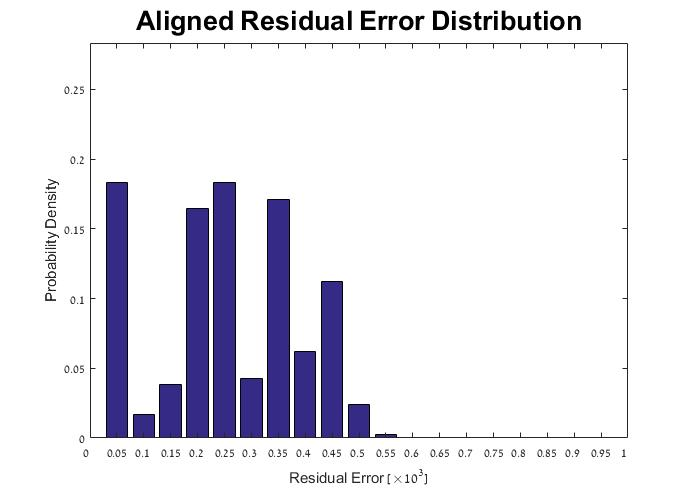
\includegraphics[width=0.48\linewidth]{figures/resError_align.jpg}
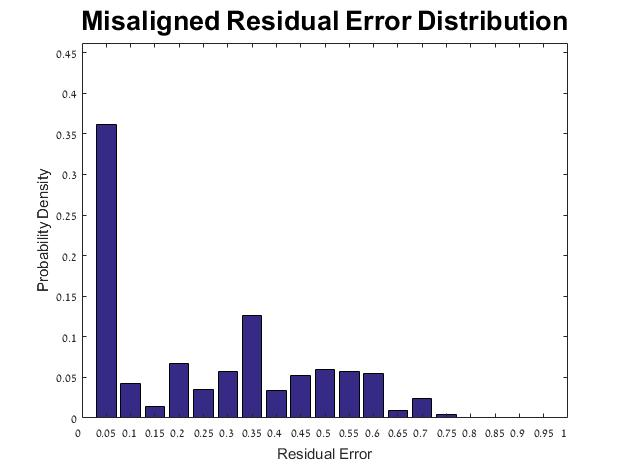
\includegraphics[width=0.45\linewidth]{figures/resError_misalign.jpg}
\caption{Aligned and misaligned latent state distributions. Data was obtained by localizing a source under varying adverse conditions (i.e. varying noise levels and T$_{60}$s. The residual error was then computed comparing the position estimate with that taken during ideal conditions (with respect to added noise). For the alignment class the microphone arrays were held static, while for the misalignment class random arrays were moved to random positions in the room.}
\label{fig:class_distributions}
\end{figure}

Specifically, we define \textbf{Z} = $\left(\textbf{z$_1$},\textbf{z$_2$},...,\textbf{z$_K$}\right)^T$ with $\textbf{z$_\textit{k}$} \in \mathbb{R}^3$ (dimensions reflect different possible latent states), $\textit{z}_{k,l} \in \{0,1\}$, and $\sum^3_{l=1}\textit{z}_{k,l} = 1$ are the latent variables, \textbf{e} = $\left(\textbf{e$_1$},\textbf{e$_2$},...,\textbf{e$_K$} \right)$ with $\textbf{e$_\textit{k}$} \in \mathbb{R}$ being the residual error associated to some sub-network of arrays, \textit{k}, with \textit{K} total sub-networks. We also define \textit{p}$\left(\textit{z$_{k,1}$} = 1\right)$, \textit{p}$\left(\textit{z$_{k,2}$} = 1\right)$, and \textit{p}$\left(\textit{z$_{k,3}$} = 1\right)$ which are the probabilities of a given sub-network being of any of the given latent states. Our task now is to estimate the posterior probabilities of the latent classes, \textit{p}$\left(\textbf{Z}\mid\textbf{e}\right)$, from which we will derive a probability of localization failure of the overall network.

We begin first by making a note regarding the priors of the residual errors. Similar to the method the authors in \cite{NA_misalignmentRecMRFsFcn} used, we estimate the prior distribution of the residual errors based off empirical data. The data was acquired by simulating an audio environment similar to what can be seen in figure 1 and proceeding as follows. We start by estimating a labelled point for all array sub-networks under ideal conditions with respect to the SNR, and also assume a T$_{60}$ of .15 (T$_{60}$s being the time it takes for the sound pressure level to reduce by 60 dB, measured after the generated test signal is abruptly ended  \cite{JS_mathDftAudioApps}). To estimate the distribution of the aligned class, we then vary the SNR (from 0dB to 40dB by increments of 2dB) and slightly vary the T$_{60}$s (between .14s and .16s by increments of .005s) and then estimate the position of a source and the resulting residual error calculated between the estimate during training under close to perfect conditions and under adverse conditions, with all arrays in the same position as they were during training. We then plot the residual errors against their relative frequency (normalized such that the output is a probability) and can see there is a correspondence between the residual error distribution with that of the normal distribution (left panel of figure 2). To estimate the distribution of the misaligned class, we perform a similar process, but instead of the arrays remaining static, for each different combination of SNR and T$_{60}$, we uniformly at random choose an array, and move it to a random position in the room. In the right panel of figure 2, we can see that the distribution of error is close to that of an exponential distribution. We note here that when plotting the residual errors, we normalize the outputs for the sake of comparison. It's also worth mentioning at this point, that we also make an assumption regarding the unknown class, namely that the distribution is uniform. The idea here is that if there is some new source, or perhaps a previous source begins to move, the frequency of error will likely be independent of the size of the error with respect to sensor alignment. It is more likely that something like the scale of disparity in location for a given source would be a much larger indicator of the residual error than the alignment of the sub-network estimates, especially if compared to the case of the aligned and misaligned states, where the residual error outcome is heavily dependent on the alignment. 

With this in mind, we now define the distributions of the priors as follows: 

\begin{equation}\label{prior distributions}
    \begin{aligned}
        \textit{p}\left(\textit{e$_k$}\mid\textit{z$_{k,1}$} = 1, \textit{$\theta_1$}\right) &= 2\mathcal{N}\left(\textit{e$_k$}; 0,\textit{$\sigma^2_\textif{A}$} \right),\\
        \textit{p}\left(\textit{e$_k$}\mid\textit{z$_{k,2}$} = 1, \textit{$\theta_2$}\right) &= \frac{\lambda\exp\{-\lambda\textit{e$_k$}\}}{1 - \exp\{-\lambda\textit{e$_{max}$}\}},\\
        \textit{p}\left(\textit{e$_k$}\mid\textit{z$_{k,3}$} = 1, \textit{$\theta_3$}\right) &= unif\left(0,\textit{e$_{max}$}\right),
    \end{aligned}
\end{equation} where \textit{e$_{max}$} is the maximum residual error, \textit{$\theta_l$} is the hyper-parameter of the \textit{l}-th likelihood distribution (i.e. $\textit{$\theta_1$} = \sigma^2_A$, $\textit{$\theta_2$} = \textit{$\lambda$}$ and $\textit{$\theta_3$} = \emptyset$).

Thus, we can now define the posterior probabilities, and note the similarity to [\ref{marginalization}]:

\begin{equation} \label{posterior_approx}
    \begin{aligned}
        \textit{p}\left(\textbf{z$_\textit{k}$}\mid\textbf{e}\right) = \sum_\textbf{z$_\textit{1}$}\cdots\sum_\textbf{z$_\textit{k-1}$}\sum_\textbf{z$_\textit{k+1}$}\cdots\sum_\textbf{z$_\textit{K}$}\textit{p}\left(\textbf{z}\mid\textbf{e} \right)
    \end{aligned}
\end{equation}

As noted above, we operate under the FCLV assumption which implies that every node receives messages from all other nodes. For the initialization process this looks like:

\begin{equation} \label{fclv_initPosterior}
    \begin{aligned}
        \textit{p}\left(\textbf{z$_k$}\mid\textbf{e}\right) = \frac{1}{\textit{Z}}\textbf{l$_\textit{k}$} \otimes \pmb{\mu}^\prime_{1 \rightarrow{\textit{k}}}\left(\textbf{z$_k$}\right) \otimes \cdots \otimes \pmb{\mu}^\prime_{k-1 \rightarrow{\textit{k}}}\left(\textbf{z$_k$}\right)\otimes \pmb{\mu}^\prime_{k+1 \rightarrow{\textit{k}}}\left(\textbf{z$_k$}\right) \cdots \otimes \pmb{\mu}^\prime_{K \rightarrow{\textit{k}}}\left(\textbf{z$_k$}\right)
    \end{aligned}
\end{equation} where \textit{Z} is a normalizing factor ensuring our posteriors are indeed probabilities, $\otimes$ is the Hadamard product, \textbf{l$_\textit{k}$} is a likelihood vector, with:

\begin{equation} \label{likelihood_vector}
    \begin{aligned}
        \textbf{l$_i$} = \left[\textit{p}\left(\textit{e$_i$}\mid\textit{z$_{i,1}$}\right), \textit{p}\left(\textit{e$_i$}\mid\textit{z$_{i,2}$}\right), \textit{p}\left(\textit{e$_i$}\mid\textit{z$_{i,3}$}\right)\right]
    \end{aligned}
\end{equation} where we've we've shortened our notation from  \textit{p}$\left(\textit{e$_k$}\mid\textit{z$_{k,l}$} = 1, \textit{$\theta_1$}\right)$ to $\textit{p}\left(\textit{e$_k$}\mid\textit{z$_{k,l}$}\right)$, and $\pmb{\mu}^\prime_{i \rightarrow{\textit{k}}}\left(\textbf{z$_k$}\right)$ is the initial message sent from the \textit{i}th to \textit{k}th hidden node and is defined as follows:

\begin{equation} \label{fclv_initMsg}
    \begin{aligned}
        \pmb{\mu}^\prime_{i \rightarrow{\textit{k}}}\left(\textbf{z$_k$}\right) = \textit{$\psi_{i,k}$}\left(\textbf{z$_i$}, \textbf{z$_k$}\right) \times \textbf{l$_i$}
    \end{aligned}
\end{equation}

After each node receives the messages from all other nodes, nodes then send messages via the following passing strategy:

\begin{equation} \label{msg_passing}
    \begin{aligned}
        \pmb{\mu}_{k-1\rightarrow{\textit{k}}}\left(\textbf{z$_k$}\right) = \textit{$\psi_{k-1,k}$}\left( \textbf{z$_{k-1}$},\textbf{z$_k$}\right)\textbf{l$_{k-1}$} &\otimes \textit{$\psi_{k-2,k-1}$}\left( \textbf{z$_{k-2}$},\textbf{z$_k-1$}\right)\textbf{l$_{k-2}$} \otimes\\& \vdots\\ &\otimes \textit{$\psi_{1,2}$}\left(\textbf{z$_1$},\textbf{z$_2$}\right)\textbf{l$_{1}$}
    \end{aligned}
\end{equation} where we note that with $\textit{k} = 1$, we compute: 

\begin{equation} \label{msg_passing_node1}
    \begin{aligned}
        \pmb{\mu}_{K\rightarrow{\textit{K-1}}}\left(\textbf{z$_K$}\right) = \textit{$\psi_{K-1,K}$}\left( \textbf{z$_{K-1}$},\textbf{z$_K$}\right)\textbf{l$_{K-1}$} \otimes \cdots \otimes\textit{$\psi_{2,3}$}\left(\textbf{z$_2$},\textbf{z$_3$}\right)\textbf{l$_{2}$}, 
    \end{aligned}
\end{equation} and the posteriors are normalized at each update such that they are in fact probabilities. Messages are passed until convergence. 

\subsection{Localization Failure Detection}
Note that we now have posteriors for a given \textit{k}th sub-network of being in any of the given hidden states, but it is still not clear how we would go about recognizing a misalignment among our sub-network estimates. Thus we now define a criterion for detecting failures based on these probabilities. We do so by defining the misalignment ratio according to \cite{NA_misalignmentRecMRFsFcn}:

\begin{equation} \label{MIS}
    \begin{alignment}
        MIS = \frac{\sum^K_{i=1}\textit{z$_{k,2}$}}{\textit{K} - \sum^K_{k=1}\textit{z$_{k,3}$}}
    \end{alignment}
\end{equation}where $\textit{z$_{k,2}$} = 1$ or $\textit{z$_{k,3}$} = 1$ denote that the \textit{k}th sensor measurement class is misaligned or unknown respectively. Naturally, we can see here that we utilize $\textit{K} - \sum^K_{k=1}\textit{z$_{k,3}$}$ in the denominator to remove array specific posteriors indicating misalignment that also have high probability of being unknown. 

We now define the probability of failure utilizing a sampling based method to approximate \textbf{$\hat{z_k}$} \backsim \textit{p}$\left(\textbf{z$_k$}\mid\textbf{e}\right)$:

\begin{equation} \label{p_failure}
    \begin{alignment}
        \textit{p$_{failure}$}\simeq\frac{1}{\textit{N}}\sum^N_{n=1}\mathbbm{1}\left(\frac{\sum^K_{i=1}\textit{$\hat{z}_{k,2}$}}{\textit{K} - \sum^K_{k=1}\textit{$\hat{z}_{k,3}$}} \geq \textbf{$\overline{MIS}$}\right)
    \end{alignment}
\end{equation} where \textbf{$\overline{MIS}$} denotes some threshold misalignment ratio (more details provided in subsequent subsection), \textit{N} is the number of sampling processes, and $\mathbbm{1}\left(\cdot\right)$ is an indicator function set at 1 when the condition within the bracket is true, and 0 if not. In practice, we run this misalignment detection algorithm every several predefined time periods. This will be more clear when we dive into more depth in detailing the overall procedure. It's worth making note here regarding the aforementioned hyper-parameters and how they were obtained. All together, the hyper-parameters we consider and that require fine tuning are $\sigma^2_\textit{A}$, $\lambda$, $\textit{$\psi_{i,j}$}\left(\textbf{z$_i$}, \textbf{z$_j$}\right)$ and \textbf{$\overline{MIS}$}. All parameters were obtained via the random search method \cite{JB_randSearchHyperParamOpt}.


%Define \textbf{l} = [p(ek|zk,1,...]
 

\section{KRLS Tracker for Time-Varying Regression}
We've now determined a way to determine if a given array has moved, and a probabilistic model to dictate which array it was that moved. We now turn to the critical task of updating the kernel covariance matrix $\Sigma_L$ after a given array has stopped moving in order to account for the fact that the labelled and unlabelled RTFs that were used in training, were recorded when the array that moved was in its original position. We begin by returning to our discussion regarding GPs. As noted, GPs are particularly nice in that they allow for easy adaptation in light of new information. This of course will be necessary in our problem, as we will need to update the covariance matrix that describes the non-linear relationship between our target function and their lower dimensional representation (i.e. RTF samples and source positions respectively). There exists a good deal of literature that details how to track non-linear, time varying relationships in data. Generally, for algorithms that are used for solving nonlinear learning programs, they typically rely on the "kernel trick", e.g. support vector machines, or kernel principal component analysis \cite{BS_learningKernelsSVMsRegOptBey}, which works well generally, but in the batch form can be unreliable due to their computational requirements. There exists a plethora of research regarding kernel-based adaptive filtering techniques that aim to mitigate these issues \cite{JK_onlineLearningWithKern, YE_kernelRlsAlgorithm, WL_kernelAdpaptiveFilterCompIntro}. The thing they all have in common, is that they try to obtain a signal of interest by adapting parameters as new data becomes available, and typically do so by minimizing a least-squares cost function. What differs is the memory and computational complexities involved. The major issue here, is that the functional representation of classical kernel-based algorithms grow linearly with the amount of processed data, meaning each update requires more memory. Naturally, this leads to the proposition of some type of forgetting mechanism, as well as reducing the amount of data needed per iteration (i.e. representing the solution using only a subset of bases that are considered relevant). One example of this was presented in \cite{WL_kernelAdpaptiveFilterCompIntro}. The authors here use an exponentially weighted kernel recursive least squares (EW-KRLS) algorithm whereby the KRLS portion of the algorithm reduces the support of the kernel to a sparse 'dictionary' of bases and a new basis is only added if it cannot be represented by a combination of other bases (i.e. if a basis becomes linearly independent) \cite{SH_adaptFilterTheory}, and the EW portion implies a forgetting factor that weighs new information exponentially more than the past. Though this algorithm does present an improvement, the problem of memory storage still exists. 

In \cite{SVV_krlsTrackTimeVaryRegr}, the authors propose an online method for solving nonlinear learning problems that is computationally efficient and effective. They in fact highlight two approaches. Firstly, they define a probabilistic framework based on Gaussian processes (GPs) that offers an intuitive view of KRLS and allows to deal with uncertainty and network regularization in a natural manner. They then propose a general strategy to forget past information based on blending the informative posterior with a non-informative distribution, and two different forgetting techniques. The first technique forgets by shifting the probability distribution over the input–output relationship toward the prior belief, converging to it once all data are forgotten, which is consistent with the Bayesian framework. The second technique forgets by gradually injecting uncertainty into older data, which, interestingly, reduces exactly to the exponentially weighted RLS algorithm when a linear kernel is used. 

For our problem at hand, we apply Van Vaerenbergh \textit{et al.}'s  online approach to updating the Gaussian kernel covariance matrix (which along with the fact that we assume our process is zero mean, fully describes the GP), and incorporate the posteriors obtained from the misalignment recognition mechanism for detecting localization failures \cite{NA_misalignmentRecMRFsFcn}. In particular, we update our inverse covariance estimate by removing basis' as described in this paper (i.e. with minimal information lost) via marginalization of the posteriors based off the KL divergence measure. Note that marginalizing out a variable in a joint Gaussian distribution is achieved by simply removing the corresponding row and column from its mean vector and covariance matrix. The difficulty however lies in deciding which time-stamped basis functions, \textit{f$_t$}, to remove. It is here that we can use the information regarding the posteriors provided via the misalignment detection FCLV-MRFs. In the author's experiments, a well-known pruning algorithm was used to determine which time based functional should be removed, where the described fixed-budget KRLS algorithm alternates the inclusion of bases and observations with the deletion of bases, using a simple basis selection and removal procedure to determine a probability of deleting any given basis. In our algorithm, we will utilize the indication of movement in the network to begin adapting the inverse covariance (precision) matrix based off position estimates from the static sub-network of microphone arrays. 

The algorithm proceeds as follows: This program iterates over time and at each iteration, determines if movement in the network occurs by comparing stored sub-network position estimates of all labelled training position with online estimates. Movement detection is done via a fully connected MRF utilizing residual errors based off sub-network positional estimates with those stored during training. If no movement occurs, no changes to the inverse covariance matrix (key in estimating source positions) occur, but position estimates are stored. If movement occurs, we estimate the position of the source using the sub-network that is still in position and movement detection is done with residual errors calculated based off positional estimates from previous iterations. This is done to ensure that once the moving array stops, we are not comparing estimates with those stored for the original array network setup. Once movement is no longer detected, we use the stored test position estimates as new labelled positions, and update the covariance matrix in a Bayesian manner to adjust for the new array positioning. We also incorporate a labelled budget, which if met, we prune our parameters. 
I.e. for the sake of saving storage space, and also incorporating a 'forgetting mechanism', such that only relevant RTF samples are used, we remove samples that yield the smallest information loss when removed.

In order to be able to calculate the pruning criterion, we must first come to understand how to update our kernel matrix and corresponding statistical parameters (i.e. the covariance function), in real time. We first note that at each time instance, we receive a new RTF observation based off of a test source that we are estimating. The RTF is utilized as a new data point and implies the total number of data points, \textit{n$_D$}, increases by 1. This of course increases the computational cost at each iteration from BLANK to BLANK. This is where the pruning method will be of use. The hypothesis is that by utilizing the pruning method to select which unlabelled RTFs should be dropped to retain accurate estimates for our points. We can measure accuracy based off estimation of labelled points. I.e., we know that the RTFs measured for all points prior to an array moving may no longer be accurate. Perhaps there are some RTF estimates where the contribution to the covariance matrix was lesser for the array that moved than for static arrays. This would mean their inclusion should still have relevance in calculating the covariance matrix.


\appendix
\section{Markov Properties}

\bibliographystyle{ieeetr}
\bibliography{bibli}

\end{document}
